\documentclass[12pt]{article}
\textwidth=17cm \oddsidemargin=-0.5cm \evensidemargin=-0.5cm
\textheight=23.7cm \topmargin=-1.4cm
\pagestyle{plain}

\usepackage{color}
\usepackage{amssymb, amsmath, amsfonts,mathrsfs,amsthm}
\usepackage{moreverb}
\usepackage{graphicx} %includegraphics[scale=#]{filename}
\usepackage{float}
\usepackage{pdfsync}
\usepackage{hyperref}  
\hypersetup{colorlinks=true}    
\usepackage{bbm}
\usepackage{tcolorbox}


\def\C{\mathbb{C}}
\def\N{\mathbb{N}}
\def\Q{\mathbb{Q}}
\def\R{\mathbb{R}}
\def\Z{\mathbb{Z}}


\begin{document}
	\title{MAT 128B: Project I}
	
	\author{Joel Aguayo, Joel Barnett, Doug Kubota, and }
	\maketitle
	
	\section{Introduction}
	Describe how we are splitting up the project here
	
	\section{Filled Julia Sets}
	\subsection{} 
	Given the function $\phi(z)=z^2+c$, where $c\in \C$ is some costant, we consider the problem of finding the fixed points of $\phi(z)$ using an iterative method. The usual process starts with some $z_0\in \C$ and uses the relation $z_{k+1}=\phi(z_k)$ to generate a sequence $\{z_n\}$ which may, or may not, converge to a fixed point of $\phi(z)$, depending on the choice of $z_0$. \\
	\newline
	Julia sets study the set of initial points which generate a converging sequence. That is, we define the filled Julia set by 
	$\{z\in \C: \text{the sequence } z_{k+1}=\phi(z_k), \text{ with initial value } z_0=z, \text{ converges}\}$, and define the Julia set to be the boundary of the filled Julia set. \\
	\newline
		We start with the simplest case: $\phi(z)=z^2$, which has two fixed points $u=1$ and $v=0$. Clearly, if $|z_0| \leq 1$, the sequence will converge because $|z_1|=|\phi(z_0)| = |(z_0)^2| \leq 1$, which implies $|z_2|\leq 1$ and so forth. Also, it is clear that if $|z_0|>1$, the sequence will diverge, because the modulus of the following terms will continue to grow. Thus, the filled Julia set for $\phi(z)$ is the unit disc $D^2=\{z: |z|\leq 1\}$, and the Julia set is the boundary of this disc. 
		
	Below is a plot of the set, which was generated with the MATLAB code provided in section \ref{code}.
	
		\begin{figure}[h!]
			\centering
			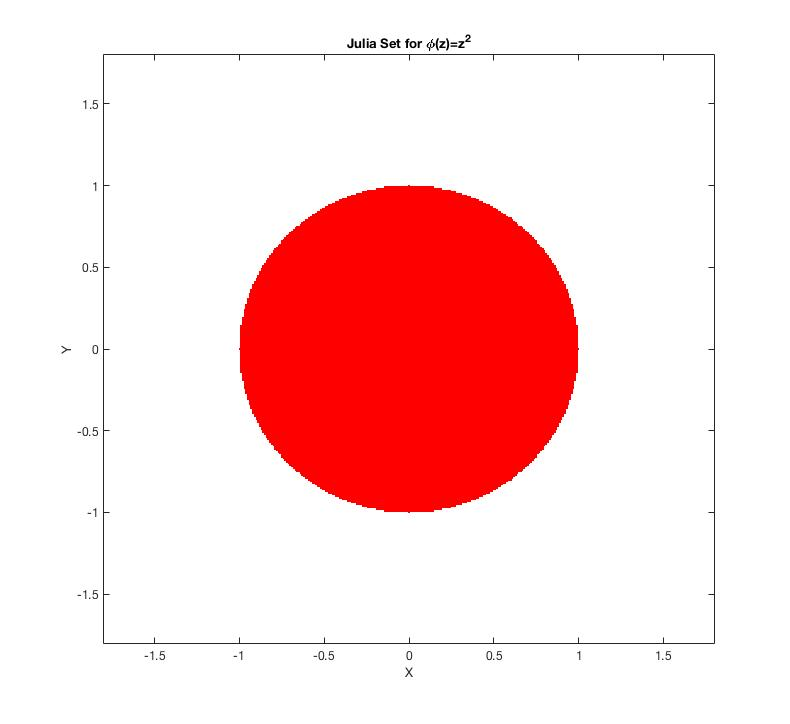
\includegraphics[width=0.6\linewidth, height=.42\textheight]{fig_1}
			\caption{}
			\label{fig:fig1}
		\end{figure}
	
	
	We also graph the Julia set for the function $\phi(z)=z^2-c$, for $c=1.25,$ $0.36+0.1i,$ $-0.123-0.745i$ and display their graph's below. 
	
	\begin{figure}[h!]
		\centering
		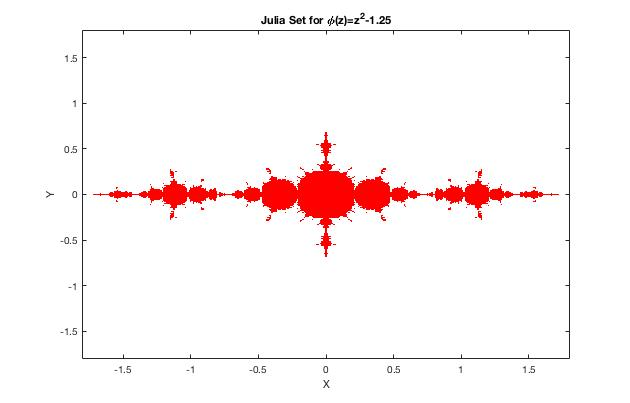
\includegraphics[width=0.7\linewidth]{Julia_Set}
		\caption{}
		\label{fig:juliaset}
	\end{figure}
	
	
	


\section{MATLAB Code} \label{code}
	
	

	
\end{document}